
% License:
% CC BY-NC-SA 3.0 (http://creativecommons.org/licenses/by-nc-sa/3.0/)
%
%%%%%%%%%%%%%%%%%%%%%%%%%%%%%%%%%%%%%%%%%

%----------------------------------------------------------------------------------------
%	PACKAGES AND OTHER DOCUMENT CONFIGURATIONS
%----------------------------------------------------------------------------------------

\documentclass[paper=a4, fontsize=11pt]{scrartcl} % A4 paper and 11pt font size

\usepackage[T1]{fontenc} % Use 8-bit encoding that has 256 glyphs
\usepackage{fourier} % Use the Adobe Utopia font for the document - comment this line to return to the LaTeX default
\usepackage[english]{babel} % English language/hyphenation
\usepackage{amsmath,amsfonts,amsthm} % Math packages
\usepackage{lipsum} % Used for inserting dummy 'Lorem ipsum' text into the template
\usepackage{enumitem}
\usepackage{caption}
\usepackage{subcaption}
\usepackage{graphicx}

\usepackage{float}

\usepackage{blindtext} %for enumarations

\usepackage[]{hyperref}  %link collor

%talbe layout to the right
%\usepackage[labelfont=bf]{caption}
%\captionsetup[table]{labelsep=space,justification=raggedright,singlelinecheck=off}
%\captionsetup[figure]{labelsep=quad}

\usepackage{sectsty} % Allows customizing section commands
\allsectionsfont{\centering \normalfont\scshape} % Make all sections centered, the default font and small caps

\usepackage{fancyhdr} % Custom headers and footers
\pagestyle{fancyplain} % Makes all pages in the document conform to the custom headers and footers
\fancyhead{} % No page header - if you want one, create it in the same way as the footers below
\fancyfoot[L]{} % Empty left footer
\fancyfoot[C]{} % Empty center footer
\fancyfoot[R]{\thepage} % Page numbering for right footer
\renewcommand{\headrulewidth}{0pt} % Remove header underlines
\renewcommand{\footrulewidth}{0pt} % Remove footer underlines
\setlength{\headheight}{13.6pt} % Customize the height of the header

\numberwithin{equation}{section} % Number equations within sections (i.e. 1.1, 1.2, 2.1, 2.2 instead of 1, 2, 3, 4)
\numberwithin{figure}{section} % Number figures within sections (i.e. 1.1, 1.2, 2.1, 2.2 instead of 1, 2, 3, 4)
\numberwithin{table}{section} % Number tables within sections (i.e. 1.1, 1.2, 2.1, 2.2 instead of 1, 2, 3, 4)

%\setlength\parindent{0pt} % Removes all indentation from paragraphs - comment this line for an assignment with lots of text


\setlength\parskip{4pt}

%----------------------------------------------------------------------------------------
%	TITLE SECTION
%----------------------------------------------------------------------------------------

\newcommand{\horrule}[1]{\rule{\linewidth}{#1}} % Create horizontal rule command with 1 argument of height

\title{	
\normalfont \normalsize 
\vspace{10pt}
\Large {Central Washington University} \\ [30pt] % Your university, school and/or department name(s)
\huge{CS567: Computational Statistics}\\ [20pt]
\huge {Project 1} \\ [20pt]
\horrule{2pt} \\[0.5cm] % Thin top horizontal rule
\Huge  Presidential Primaries\\ % The assignment title
\horrule{2pt} \\[1cm] % Thick bottom horizontal rule
\Large{Submitted By} \\ [0.01cm]


\newline
\huge{Andrew Dunn}\\[0.05cm]
\newline
\huge{Justin Phan Phan}\\[0.05cm]
\newline
\huge{Mark Sichong}\\[0.05cm]
\newline 
\huge{Sridevi Wagle}\\ [0.05cm]
\newline
\vspace{1cm}

\includegraphics[width=30mm,height=30mm]{Logo.PNG}\\[0.1cm]
\Large{March 5, 2020}\\ [0.6cm]
\date{}
}

\begin{document}
%\nocite{*}
\maketitle % Print the title
\tableofcontents

%----------------------------------------------------------------------------------------
%	Sections
%----------------------------------------------------------------------------------------

\section{Introduction}
\subsection{Brief Introduction}
For this project we applied basic statistical methods to the 2019-2020 Democratic Primary election cycle. An election for the President of the United States happens every four years and is the largest political event in the USA. Leading up to the general election, most of the candidates running for president go through a series of state primaries and caucuses. Although these primaries and caucuses are ran differently, they both serve the same purpose. They allow every state to choose their major political parties’ nominees for the general election\cite{usagov}. The campaigning process lasts at least a year for most candidates and costs many millions of dollars in advertising outreach, and travelling. Since the Republican Presidential Nominee is almost guaranteed to be President Donald Trump, we focused on the Democratic Nominee Primaries. Below you will find the list of objectives used in this project:

\subsection{Objectives}
\begin{itemize}
    \item To monitor polling data for the Democratic Party primary candidates
    \item To read the polling data from source into a R dataframe, filter and plot polling data over time and to run analysis and prediction tools using R script 
    \item To plot the fundraising for Democratic candidates
    \item To plot the number of delegates awarded for candidates (state wise)
\end{itemize}

% \subsection{Dataset}
% \begin{itemize}
%     \item Dataset from fivethirtyeight.com\cite{jr._malone_skelley_koerth_paine_dubin_sawchik_rakich} is used in this project and website tracks a large number of different polls
%     \item  The data is available in a csv format and updated on a regular basis. 
%     \item The csv file includes columns like pollster name, state, sponsor, sample size, source, poll start and end dates and poll results as a percentage of votes for each candidate
% \end{itemize}

\section{Design}\label{design}

\subsection{Data Set}

All of the polling data used in our analysis was downloaded from FiveThirtyEight, a well known political blog that does predictions for various elections. They collect polling data from a large number of different pollsters and then combine all into a single $.csv$ file that is available for download. In addition, FiveThirtyEight rates all pollsters based on their quality and level of bias. Ratings range from A+ down to F. Pollsters with the least bias have the best ratings. Using their ratings, we are able to filter the data set such that only highly rated polls are considered. Other than polling data, FiveThirtyEight presents many other aspects of the election we can analyze such as candidate funding and number of delegates.

\subsection{Implementation}

For our experiments we implemented a program in R that can import the data set and generate various plots of the polling data. Using these plots we can visualize the data and conduct some analysis, looking for trends.
\section{Analysis}\label{analysis}

\subsection{Analysis of Delegates}

Figure \ref{Delegate} shows the total number of delegates gathered by each of the major candidates, grouped by state. It is clear based on this graph alone that Biden and Sanders seem to be the two main candidates that have a chance at winning the Democratic Presidential Nomination. Biden appears to be more successful in south eastern states such as North Carolina, South Carolina, and Alabama, while Sanders tends to be more successful in west and mid-western states such as California, Nevada, and Colorado.

\subsection{Analysis of Polling Data}

Looking at figure \ref{Updated-Polling-Data-1}, you will see the average candidate polling support over time. The data is from all A-rated polls collected by FiveThirtyEight. According to this graph, Senator Sanders leads the way. His average support is the highest. Joe Biden's support varies more and is ranked second most of time. Bloomberg, Buttigieg, and Warren are all are fighting for third place, but none of the three clearly come out on top. Pete Buttigieg is one of the youngest candidates, and his achievements in his hometown really changed that city. Looking at poll results however, we can see that his influence and movement is not greatly affecting people outside his city. Starting from middle of February, his was support steadily decreased. Comparing with recent news, the graph is correct. Buttigieg, Warren, and Bloomberg have all dropped out. Biden and Sanders will compete for the last position.

Figure \ref{A-rated-polls} contains the same A-rated polling data as figure \ref{Updated-Polling-Data-1}, but is focused around the various primary and caucus events leading up to super tuesday. For most of the time series displayed, Senator Sanders ranked first in support. Although he lost some support following the 9th Presidential Debate, the polls bounced back leading up to the South Carolina Primary. Joe Biden's support rate dropped starting from Feb. 25 following the widely televised "dog-faced pony tail soldiers" insult that he spoke to a college girl. However his rate rebounded at Feb. 29 following the South Carolina Primary. During this time frame Bloomberg trades blows with Biden before settling in around third place with Warren. Finally, Buttigieg's support appears to steadily decrease before sharply declining, leading up to him dropping out of the race on Feb. 29. Note that at the time of writing for this report, there was no data available for A-rated polls on super tuesday.

Due to the lack of polling data from super tuesday, we also plotted the averages of all polls, regardless of their rating, which you can see in figure \ref{All-rated-polls}. This gives us a little more data, showing poll results up to super tuesday. In this graph we can see that Biden overtakes Sanders in average support right before super tuesday. Again Bloomberg and Warren are tied in third place, with Buttigieg coming last.

Figures \ref{scatter-A-rated}, \ref{scatter-all}, and \ref{scatter-all-linear} display the polling data as a scatter plot with regression lines. The shaded grey areas represent the $95\%$ confidence interval's for each candidate. These plots only contain the the primary candidates left in the race at the time of analysis. As you can see from the scatter plots, there is a large variation in polling results, even among the A-rated polls. This large variation makes accurate predictions very difficult. In addition, there is a difference in trends between figures \ref{scatter-A-rated} and \ref{scatter-all}. In figure \ref{scatter-A-rated}, only the A-rated polls are plotted. Here it appears that both Sanders and Biden's level of support is declining after the South Carolina Primary. In contrast, figure \ref{scatter-all} contains polling data from all polls and shows the opposite trend. Now both Sanders and Biden show an increasing level of support leading up to and after the South Carolina Primary, with Biden's support increasing faster than Sanders. Figure \ref{scatter-all-linear} shows the same set of polls but displays a linear regression. This graph shows the same general trend as figure \ref{scatter-all}, where both Sanders and Biden have an ever increasing level of support. The discrepancies between polls make accurate predictions based on simple regression lines near impossible.

\subsection{Analysis of Ad Spending and Funding}


\section{Model}\label{model}
\begin{figure}[H]
    \centering
    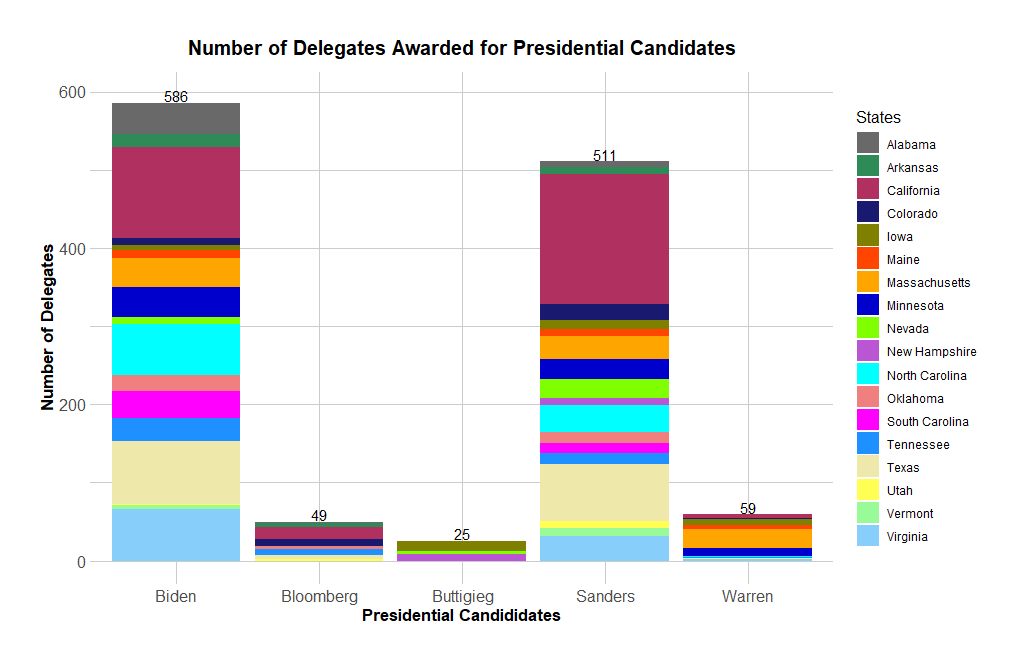
\includegraphics[width=0.9\textwidth]{C:/Users/phanho/Desktop/Project1cs565/CS567_Pres_Primary/Delegate.png}
    \caption{Delegate}
    \label{Delegate}
\end{figure}
\begin{figure}[H]
    \centering
    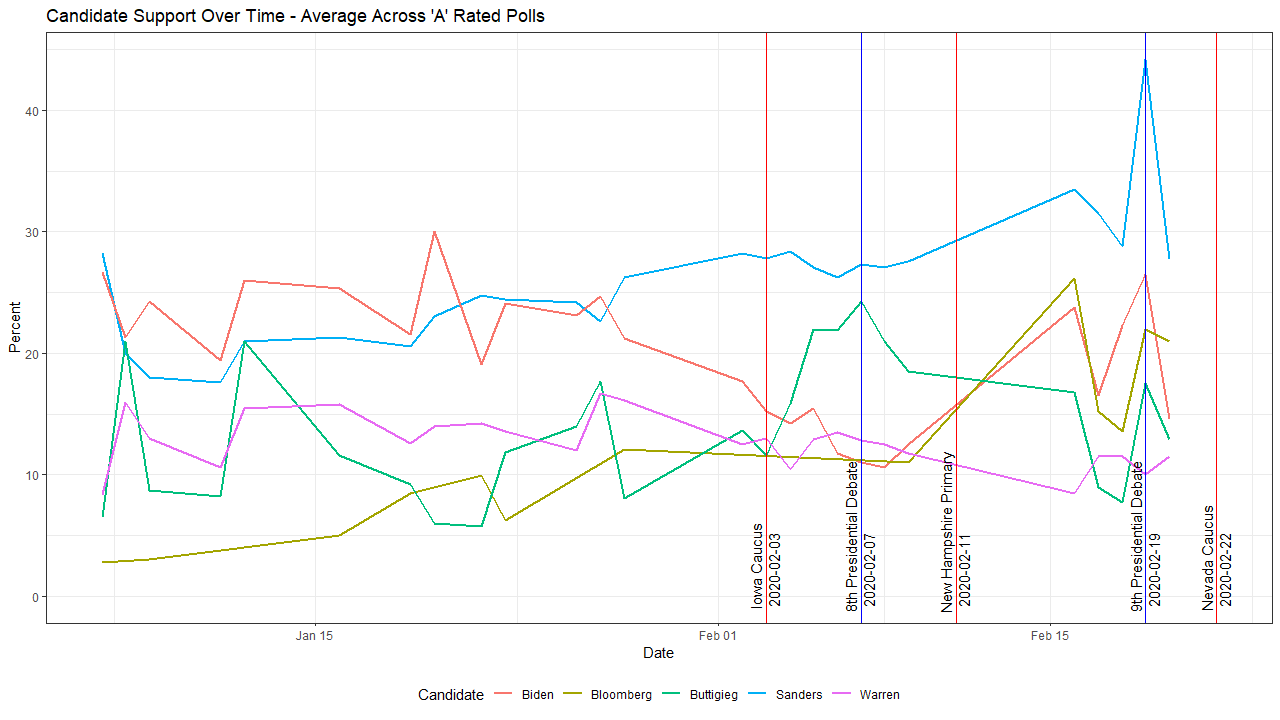
\includegraphics[width=0.9\textwidth]{C:/Users/phanho/Desktop/Project1cs565/CS567_Pres_Primary/long-A-rated-polls.png}
    \caption{Updated Polling Data 1 }
    \label{Updated-Polling-Data-1}
\end{figure}
\begin{figure}[H]
    \centering
    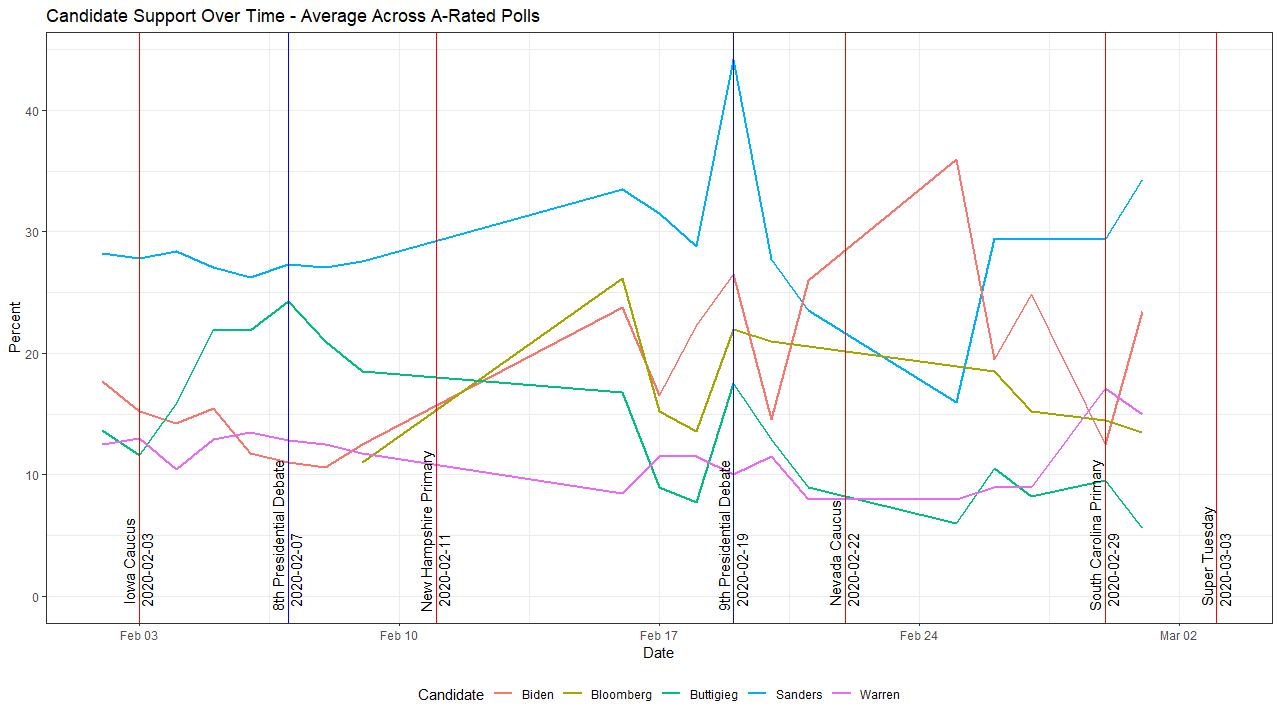
\includegraphics[width=0.9\textwidth]{C:/Users/phanho/Desktop/Project1cs565/CS567_Pres_Primary/A-rated-polls.png}
    \caption{A-rated-polls}
    \label{A-rated-polls}
\end{figure}
\begin{figure}[H]
    \centering
    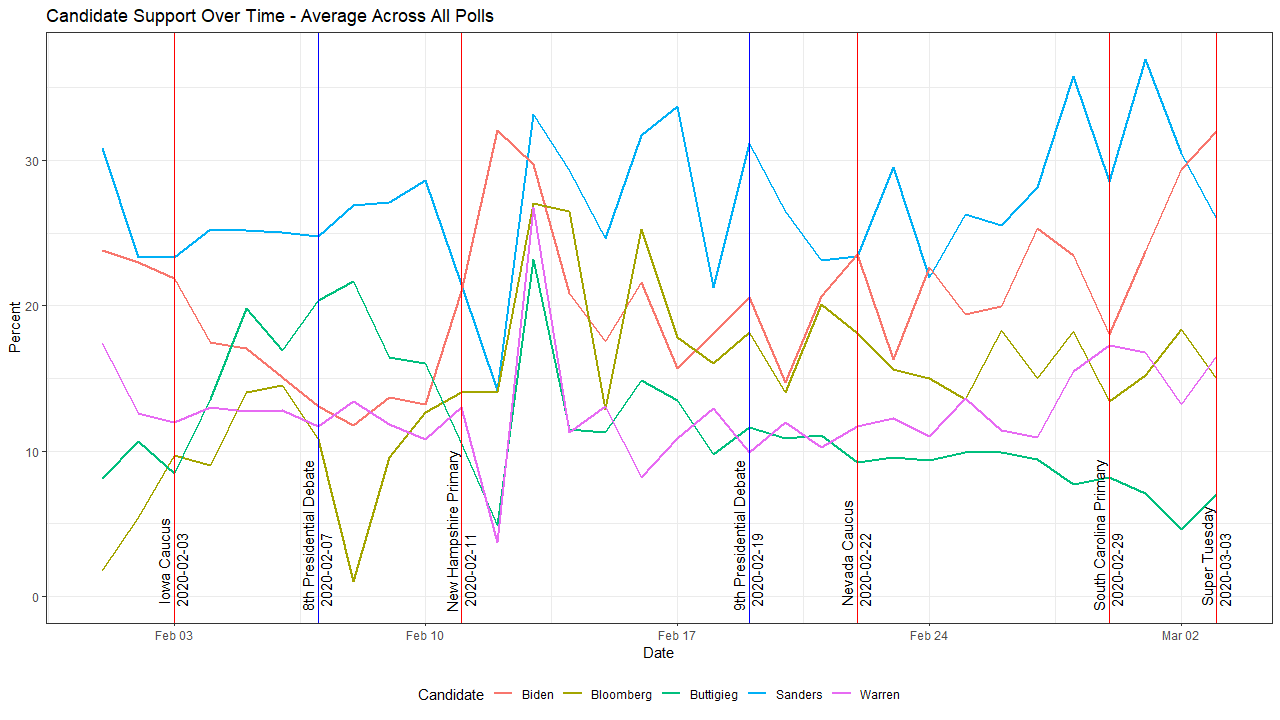
\includegraphics[width=0.9\textwidth]{C:/Users/phanho/Desktop/Project1cs565/CS567_Pres_Primary/All-rated-polls.png}
    \caption{All-rated-polls}
    \label{All-rated-polls}
\end{figure}
\begin{figure}[H]
    \centering
    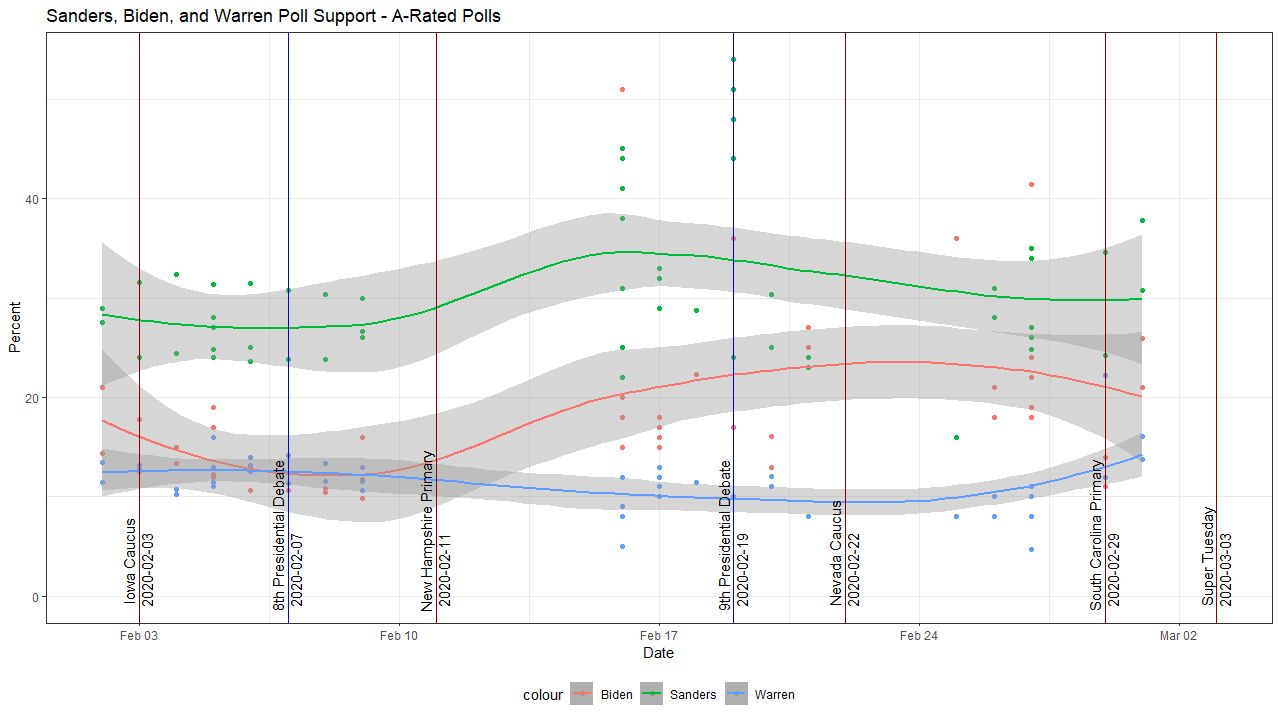
\includegraphics[width=0.9\textwidth]{C:/Users/phanho/Desktop/Project1cs565/CS567_Pres_Primary/scatter-A-rated.png}
    \caption{scatter-A-rated}
    \label{scatter-A-rated}
\end{figure}
\begin{figure}[H]
    \centering
    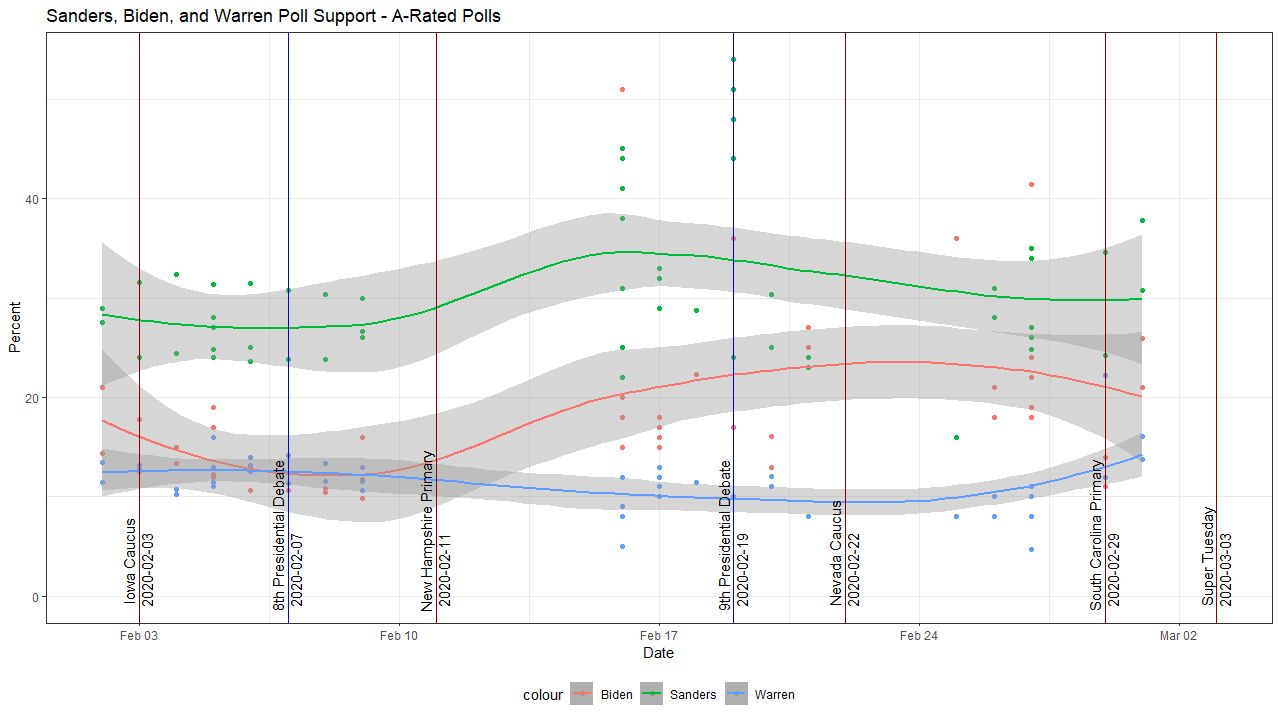
\includegraphics[width=0.9\textwidth]{C:/Users/phanho/Desktop/Project1cs565/CS567_Pres_Primary/scatter-A-rated.png}
    \caption{scatter-A-rated}
    \label{scatter-A-rated}
\end{figure}
\begin{figure}[H]
    \centering
    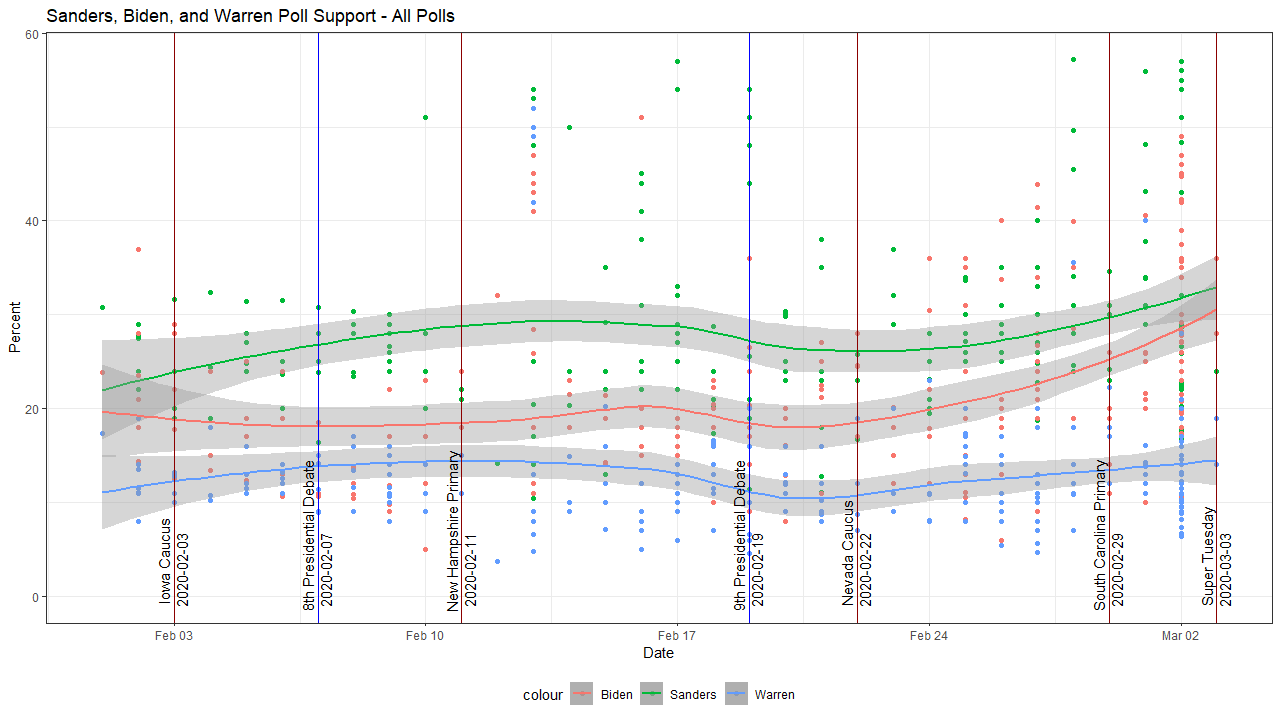
\includegraphics[width=0.9\textwidth]{C:/Users/phanho/Desktop/Project1cs565/CS567_Pres_Primary/scatter-all.png}
    \caption{scatter-all}
    \label{scatter-all}
\end{figure}
\begin{figure}[H]
    \centering
    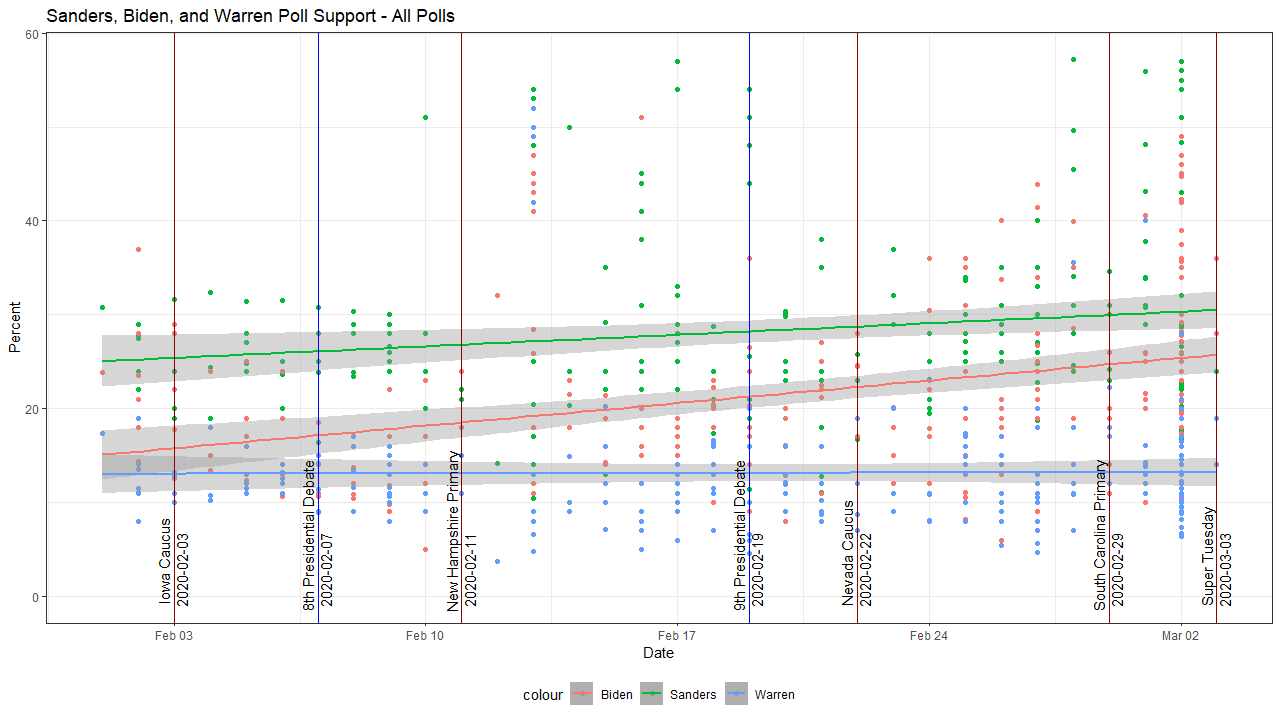
\includegraphics[width=0.9\textwidth]{C:/Users/phanho/Desktop/Project1cs565/CS567_Pres_Primary/scatter-all-linear.png}
    \caption{scatter-all-linear}
    \label{scatter-all-linear}
\end{figure}
\begin{figure}[H]
    \centering
    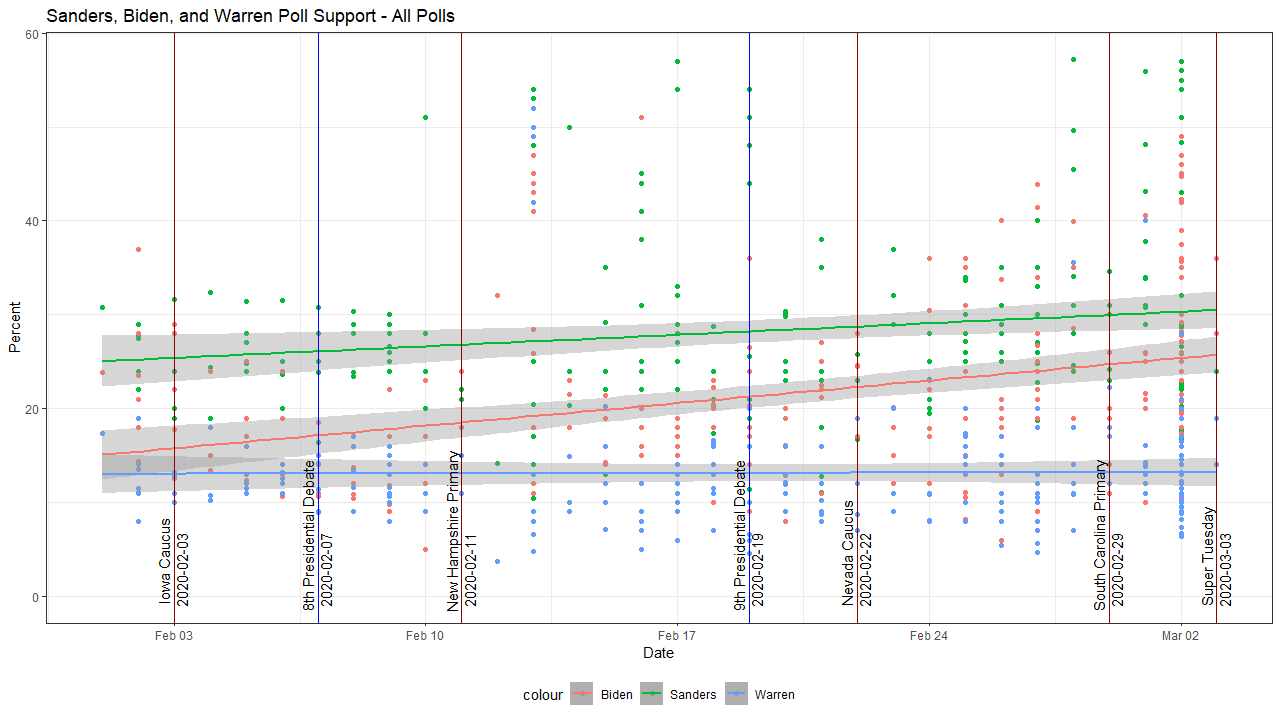
\includegraphics[width=0.9\textwidth]{C:/Users/phanho/Desktop/Project1cs565/CS567_Pres_Primary/scatter-all-linear.png}
    \caption{scatter-all-linear}
    \label{scatter-all-linear}
\end{figure}
\begin{figure}[H]
    \centering
    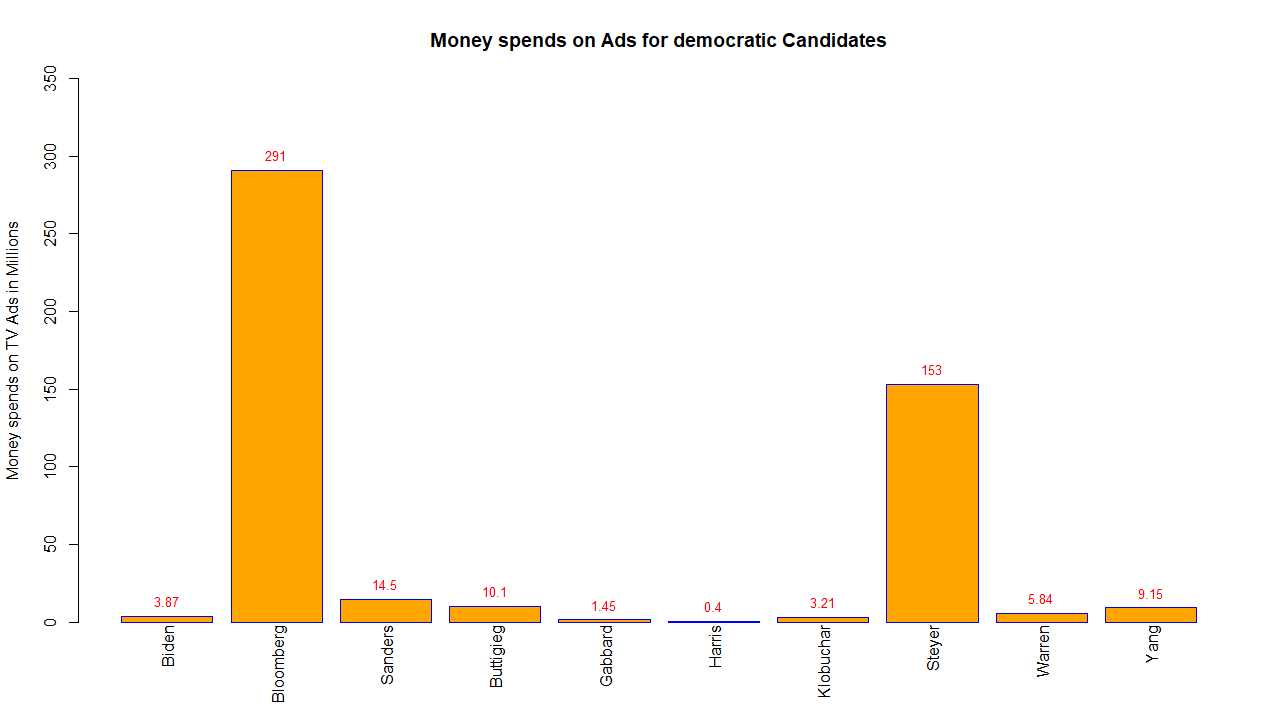
\includegraphics[width=0.9\textwidth]{C:/Users/phanho/Desktop/Project1cs565/CS567_Pres_Primary/MoneyspendinAds.png}
    \caption{Money spending on Ads}
    \label{MoneyspendinAds}
\end{figure}
\begin{figure}[H]
    \centering
    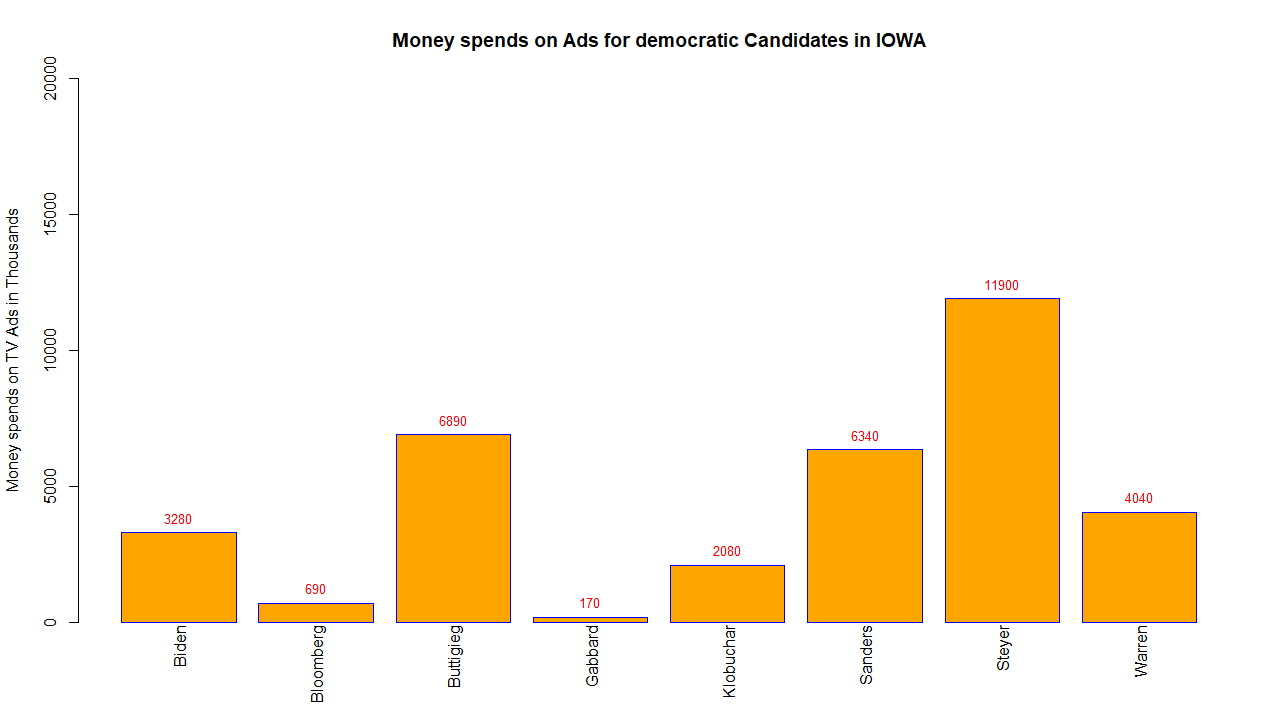
\includegraphics[width=0.9\textwidth]{C:/Users/phanho/Desktop/Project1cs565/CS567_Pres_Primary/IOWA.png}
    \caption{Money spending on Ads in Iowa}
    \label{IOWA}
\end{figure}

\begin{figure}[H]
    \centering
    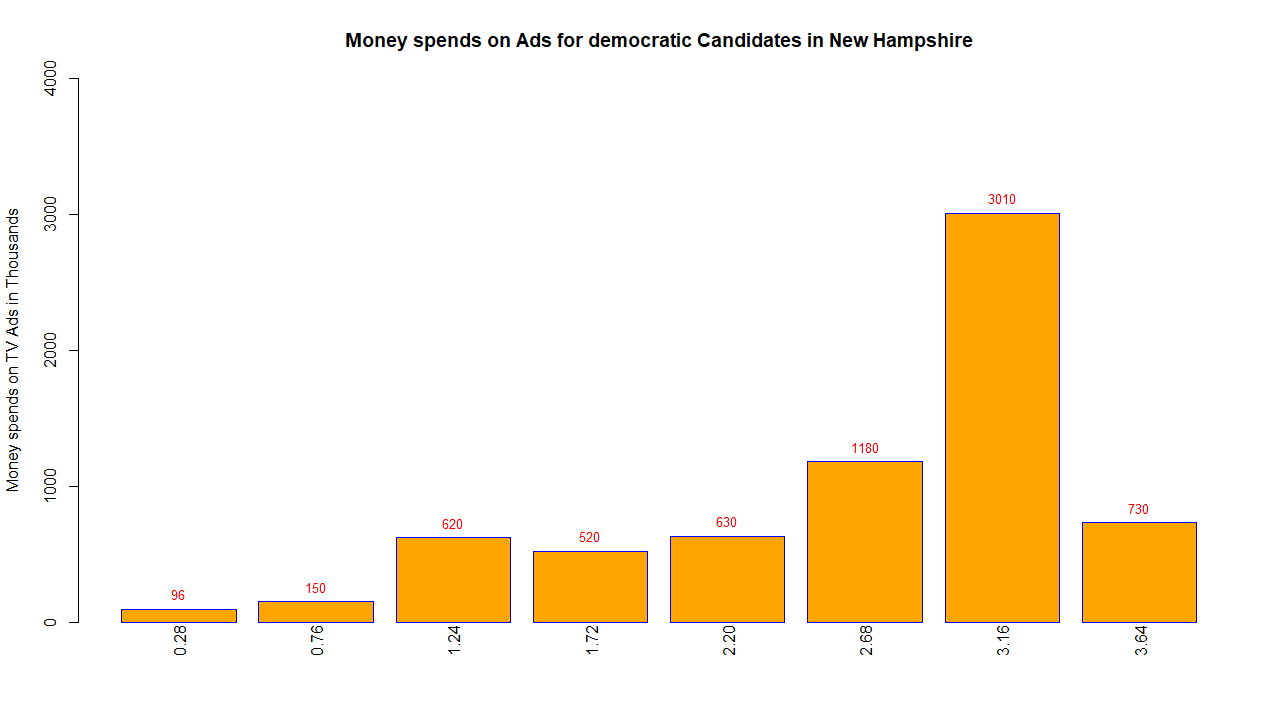
\includegraphics[width=0.9\textwidth]{C:/Users/phanho/Desktop/Project1cs565/CS567_Pres_Primary/Newhampshire.png}
    \caption{Money spending on Ads in New Hampshire}
    \label{Newhampshire}
\end{figure}
\begin{figure}[H]
    \centering
    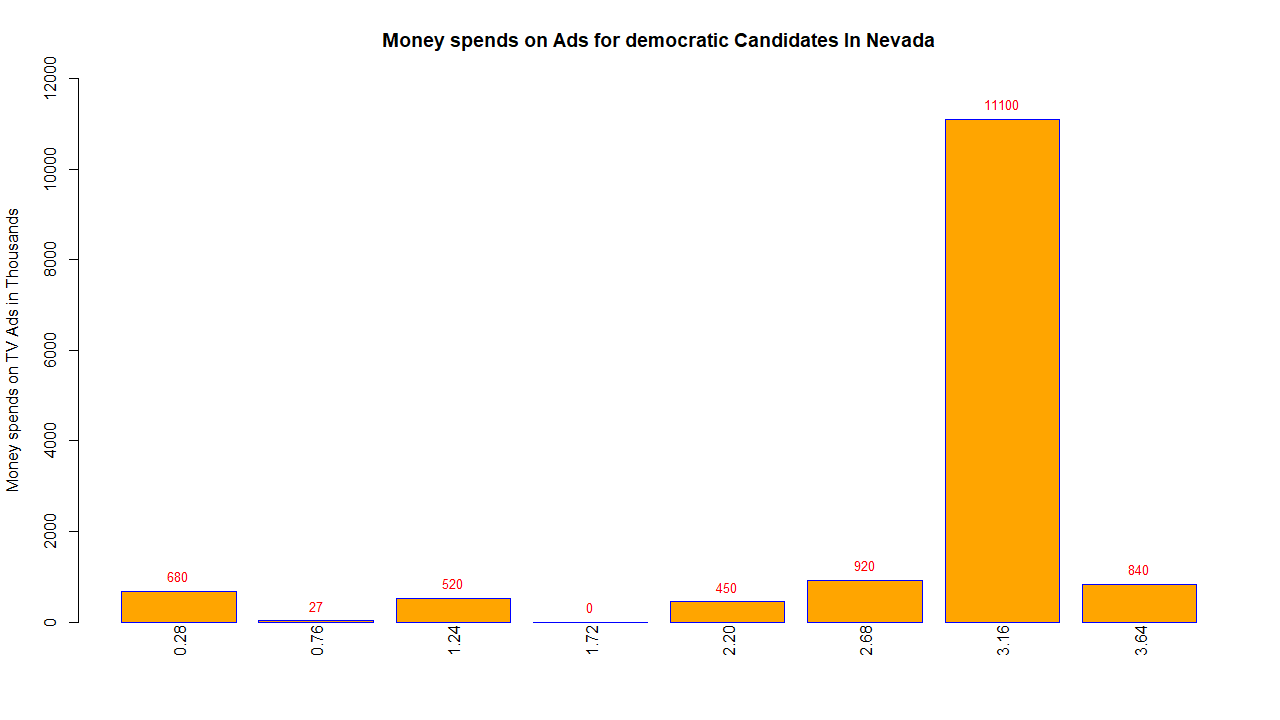
\includegraphics[width=0.9\textwidth]{C:/Users/phanho/Desktop/Project1cs565/CS567_Pres_Primary/Nevada.png}
    \caption{Money spending on Ads in Nevada}
    \label{Nevada}
\end{figure}
\begin{figure}[H]
    \centering
    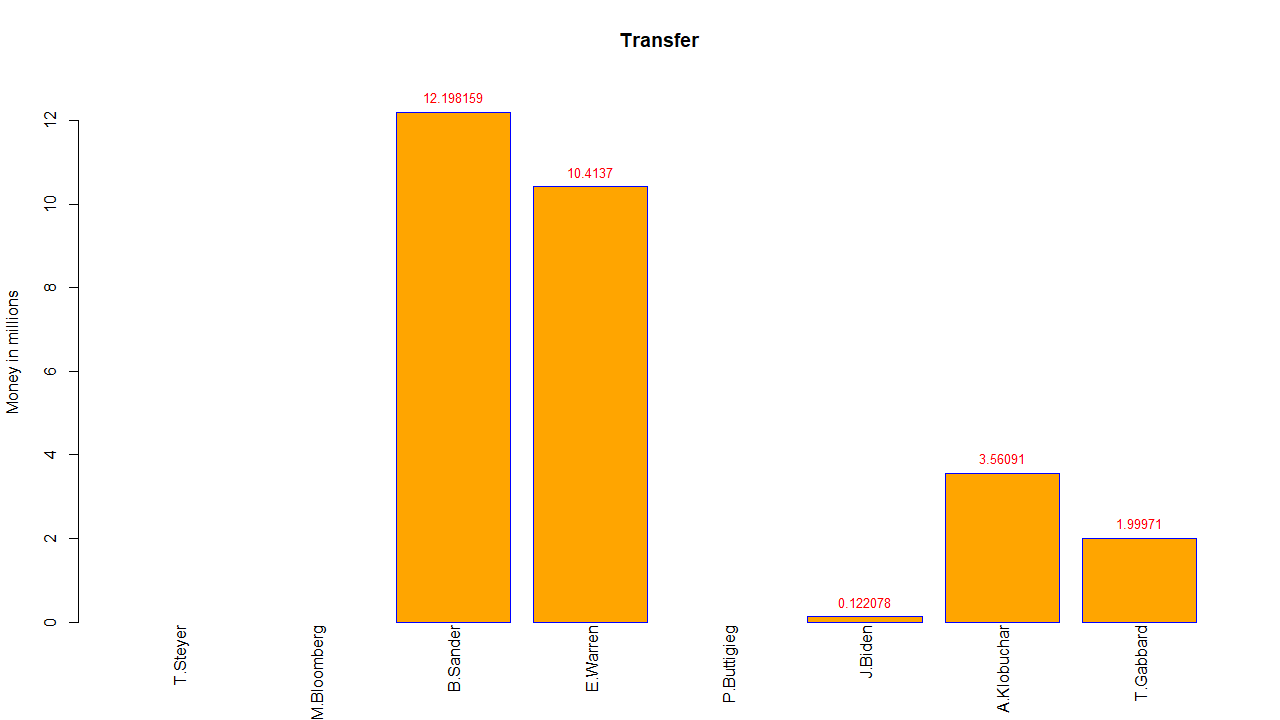
\includegraphics[width=0.9\textwidth]{C:/Users/phanho/Desktop/Project1cs565/CS567_Pres_Primary/Total.png}
    \caption{Total Funding}
    \label{Total}
\end{figure}
\begin{figure}[H]
    \centering
    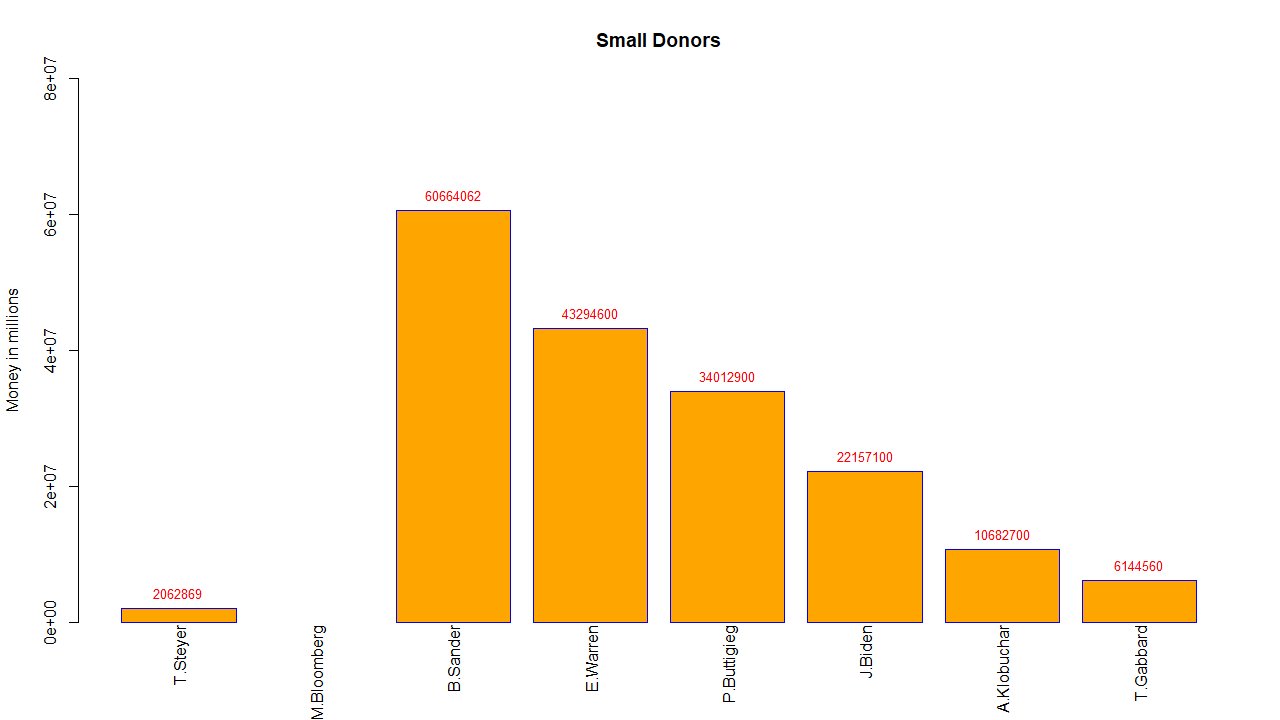
\includegraphics[width=0.9\textwidth]{C:/Users/phanho/Desktop/Project1cs565/CS567_Pres_Primary/Small Donors.png}
    \caption{Small Donors Funding}
    \label{Small Donors}
\end{figure}
\begin{figure}[H]
    \centering
    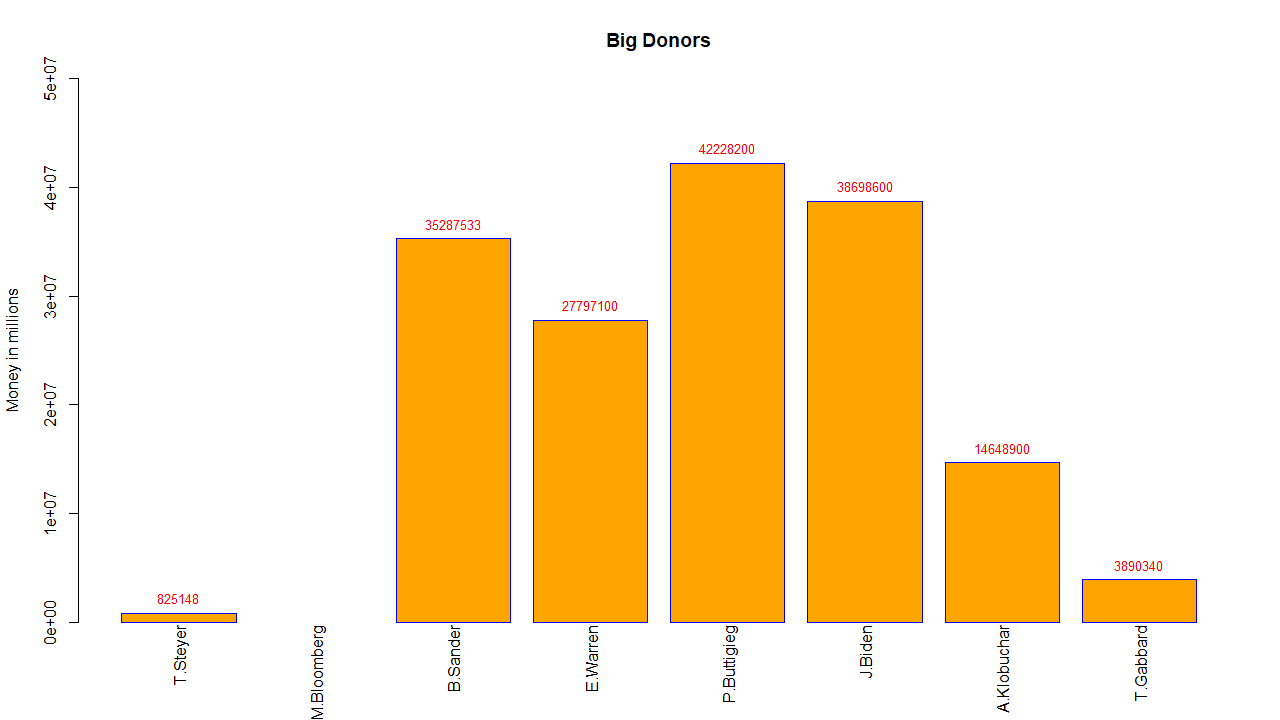
\includegraphics[width=0.9\textwidth]{C:/Users/phanho/Desktop/Project1cs565/CS567_Pres_Primary/Bigdonor.png}
    \caption{Big donors Funding}
    \label{Bigdonor}
\end{figure}
\begin{figure}[H]
    \centering
    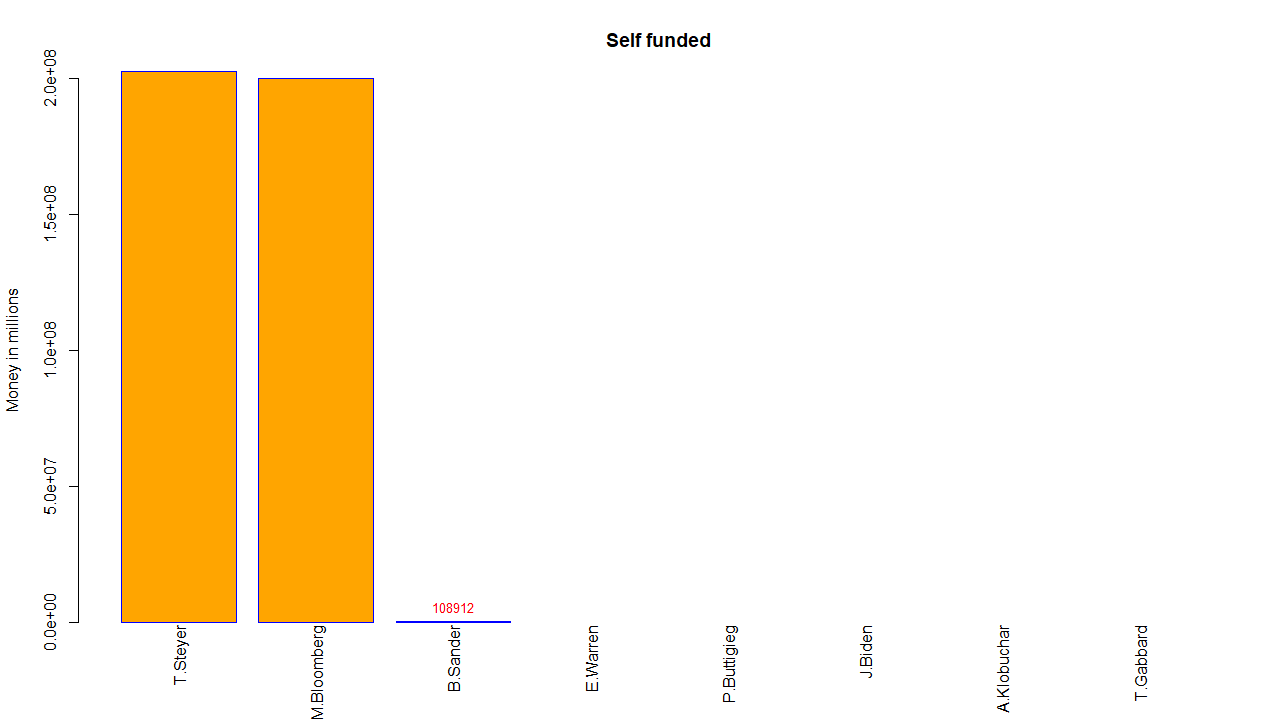
\includegraphics[width=0.9\textwidth]{C:/Users/phanho/Desktop/Project1cs565/CS567_Pres_Primary/Selffunnded.png}
    \caption{Self funnded Funding}
    \label{Selffunnded}
\end{figure}
\begin{figure}[H]
    \centering
    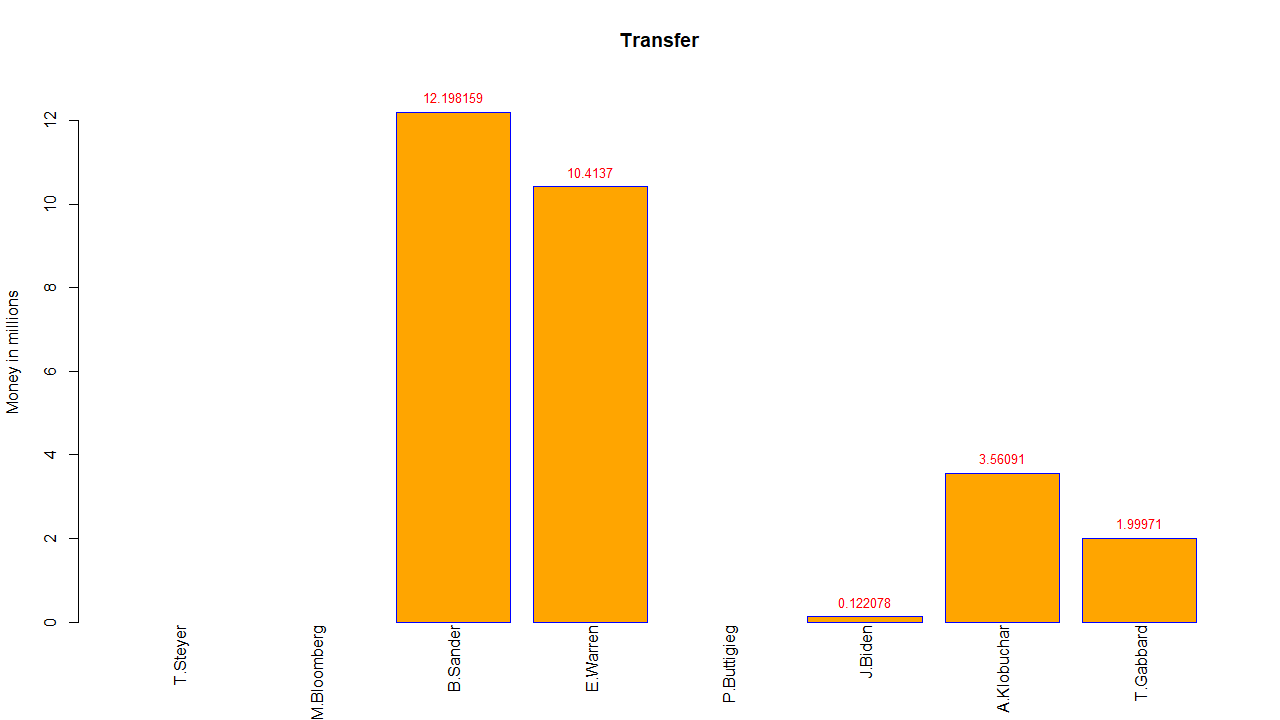
\includegraphics[width=0.9\textwidth]{C:/Users/phanho/Desktop/Project1cs565/CS567_Pres_Primary/Transfer.png}
    \caption{Transfer Funding}
    \label{Transfer}
\end{figure}
Others
\begin{figure}[H]
    \centering
    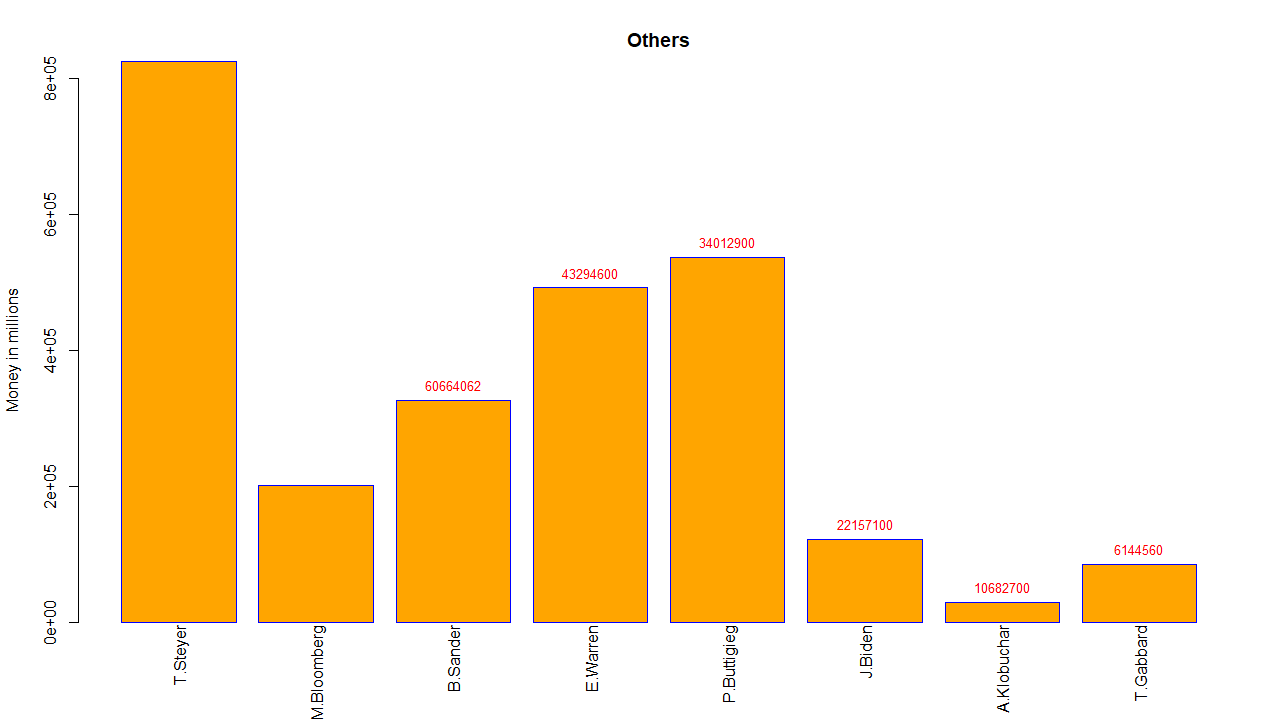
\includegraphics[width=0.9\textwidth]{C:/Users/phanho/Desktop/Project1cs565/CS567_Pres_Primary/Others.png}
    \caption{Others Sources Funding}
    \label{Others}
\end{figure}
\input{conclusion}



%bibliography


\end{document}